%%%%%%%%%%%%%%%%%%%%%%%%%%%%%%%%%%%%%%%%%
%
% (c) 2022 by Jennifer Laaser
%
% This work is licensed under the Creative Commons Attribution-NonCommercial-ShareAlike 4.0 International License. To view a copy of this license, visit http://creativecommons.org/licenses/by-nc-sa/4.0/ or send a letter to Creative Commons, PO Box 1866, Mountain View, CA 94042, USA.
%
% The current source for these materials is accessible on Github: https://github.com/jlaaser/pogil-polymers
%
%%%%%%%%%%%%%%%%%%%%%%%%%%%%%%%%%%%%%%%%%

\renewcommand{\figpath}{content/polymchem/stepgrowth/dispersity/figs}
\renewcommand{\labelbase}{step-dispersity}

\begin{activity}{Molecular Weight Distributions in Step-Growth Polymerizations}

\begin{instructornotes}

	This activity introduces students to key concepts related to the molecular weight distributions obtained in step-growth polymerizations.
	
	After completing this activity, students will be able to:
			\begin{enumerate}
				\item Calculate the fraction of polymer chains with length $i$ in a step-growth polymerization,
				\item Describe, qualitatively, the chain length distribution and how it changes with extent of reaction,
				\item Calculate the expected dispersity for a step-growth polymerization at a given extent of reaction, and
				\item Explain why the limiting dispersity for a step-growth polymerization is 2.
			\end{enumerate}
			
	\subsection*{Activity summary:}
	\begin{itemize}
		\item \textbf{Activity type:} Learning Cycle
		\item \textbf{Content goals:} See above
		\item \textbf{Process goals:} %https://pogil.org/uploads/attachments/cj54b5yts006cklx4hh758htf-process-skills-official-pogil-list-2015-original.pdf
			\begin{itemize}
				\item Interpretation and application of a mathematical model
				\item Analysis of numerical and graphical data
				\item Written and oral communication of reasoning
			\end{itemize}
		\item \textbf{Duration:} 25-30 minutes, including time for discussion
		\item \textbf{Instructor preparation required:} none beyond knowledge of relevant content
		\item \textbf{Related textbook chapters:}
			\begin{itemize}
				\item \emph{Polymer Chemistry} (Hiemenz \& Lodge), 2nd ed.: section 2.4
				\item \emph{Introduction to Polymers} (Young \& Lovell), 3rd ed.: section 3.2.3.2
			\end{itemize}
	\end{itemize}

\end{instructornotes}

	%\textbf{Focus question:} Put a central question for the students to consider through this exercise here.

\begin{model}[Probabilities of Forming Different Chain Lengths]
\label{\labelbase:mdl:probabilities}

Recall that in a step-growth polymerization of AB-type monomers, the extent of reaction $p$ gives the fraction of `A' groups that have reacted.

In terms of probabilities, the \emph{probability} that a particular `A' group reacts (turns into an `a' group) is $p$, while the probability that it \emph{does not} react (remains an `A' group) is $1-p$:

	\centerline{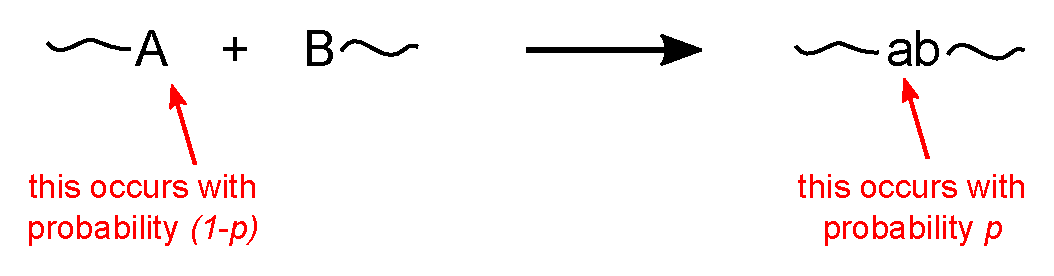
\includegraphics[width=0.7\textwidth]{\figpath/model1-rxn}}

	Each molecule has some combination of unreacted `A' groups and reacted `a' groups, each of which occurs with probability $p$ or $(1-p)$ as appropriate:

	\centerline{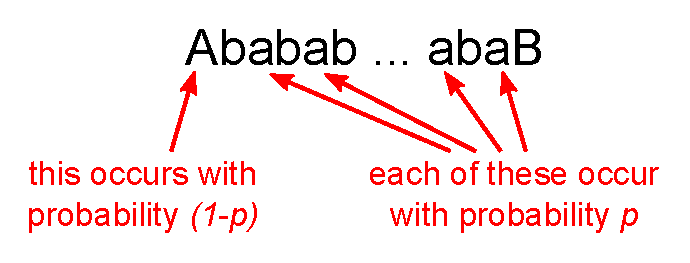
\includegraphics[width=0.5\textwidth]{\figpath/model1-molecule}}
	
	The \emph{total} probability of forming this molecule is just the product of the probabilities for each group:
	\begin{equation*}
		P(molecule) = \underbrace{(p \times p \times p \times \dots)}_{\text{one factor of p for each reacted `a' group}} \times \underbrace{((1-p) \times (1-p) \times \dots)}_{\text{one factor of (1-p) for each unreacted `A' group}} 
	\end{equation*}
or, more concisely,
	\begin{equation*}
		P(molecule) = p^\text{(number of reacted `a' groups)}\times(1-p)^\text{(number of unreacted `A' groups)}
	\end{equation*}


\end{model}

\vspace{0.05in}
\begin{ctqs}
	
	\question Consider an AbabaB trimer:
		\begin{enumerate}
			\item How many monomers came together to form this molecule (that is, what is its degree of polymerization)?
			
				\begin{solution}[0.5in]{}
					3
				\end{solution}
				
			\item How many \emph{unreacted} `A' groups are in this molecule?
			
				\begin{solution}[0.5in]{}
					1
				\end{solution}
				
			\item How many \emph{reacted} `a' groups are in this molecule?
			
				\begin{solution}[0.5in]{}
					2
				\end{solution}
				
			\item What is the probability of forming an AbabaB trimer?
			
				\begin{solution}[0.5in]{}
					$P(AbabaB) = p^\text{number of reacted a groups}(1-p)^\text{number of unreacted A groups} = p^2(1-p)^1 = p^2(1-p)$
				\end{solution}
				
		\end{enumerate}
		
	\question More generally, consider a molecule with degree of polymerization $i$ (that is, a molecule that was made by linking together $i$ AB-type monomers).
	
		\begin{enumerate}
		
			\item How many \emph{unreacted} `A' groups are in this molecule?
			
				\begin{solution}[0.5in]{}
					1
				\end{solution}
				
			\item How many \emph{reacted} `a' groups are in this molecule?
			
				\begin{solution}[0.5in]{}
					i-1
				\end{solution}
				
			\item What is the probability of forming a molecule with degree of polymerization $i$?
			
				\begin{solution}[1in]{}
					$P(i-mer) = p^\text{number of reacted a groups}(1-p)^\text{number of unreacted A groups} = p^{i-1}(1-p)^1 = p^{i-1}(1-p)$
				\end{solution}
			
		\end{enumerate}
		
\end{ctqs}

\begin{infobox}
	The \emph{probability} that a molecule has degree of polymerization $i$ is the same as the \emph{fraction of molecules} that have degree of polymerization $i$.
\end{infobox}


\begin{ctqs}
	
	\question Complete the following statement:
	
		``The fraction of molecules, $x_i$, that have degree of polymerization $i$ is \line(1,0){50}.''
	
		\begin{solution}[0.75in]{}
		
			$x_i = p^{i-1}(1-p)$
			
		\end{solution}
		
\end{ctqs}

\begin{model}[Chain Length Distributions]
\label{\labelbase:mdl:dist}

	The following table gives selected values of $x_i$ calculated at two different extents of reaction, $p$, using the expression you derived in Model \ref{\labelbase:mdl:probabilities}:
	
		\begin{center}
			\renewcommand{\arraystretch}{1.5}
			\begin{tabular}{ccc}
				\hline
				\textbf{~~$i$~~} & ~~~$x_i$ when $p=0.5$~~~ & ~~~$x_i$ when $p=0.9$~~~ \\\hline
				1 & 0.5 & 0.1 \\
				2 & 0.25 & 0.09 \\
				3 & 0.125 & 0.08 \\
				5 & 0.0313 & 0.065 \\
				10 & 9.7x10$^{-4}$ & 0.0387 \\
				15 & 3.1x10$^{-5}$ & 0.0229 \\
				20 & 9.5x10$^{-7}$ & 0.0135 \\\hline
			\end{tabular}
		\end{center}
		
		\vspace{0.1in}

\end{model}
	
\begin{ctqs}

	\question Plot the data given in Model \ref{\labelbase:mdl:dist} on the following axes.  Make sure to use a different symbol for points corresponding to $p=0.5$ than for the points corresponding to $p=0.9$.
	
		\begin{solution}[3.25in]{%
				\centerline{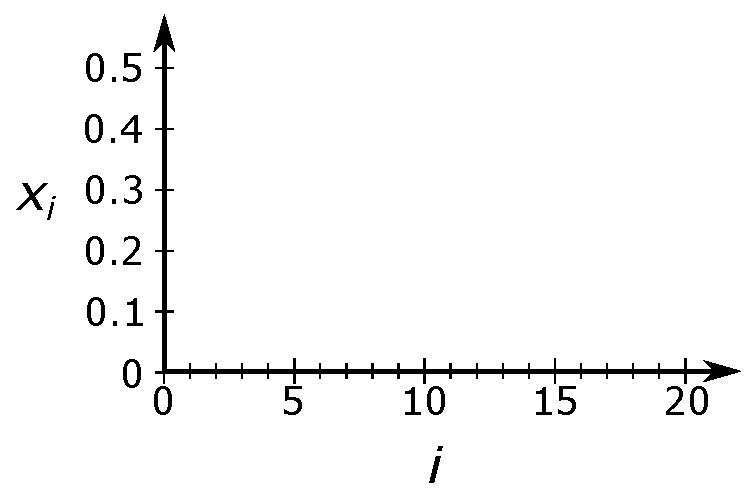
\includegraphics[width=0.8\textwidth]{\figpath/model2-xi-axes.pdf}}
			}
				\centerline{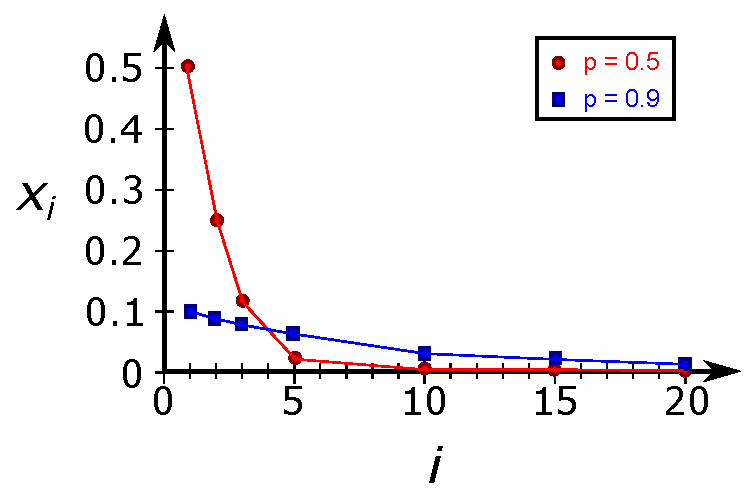
\includegraphics[width=0.8\textwidth]{\figpath/model2-xi-plotted.pdf}}
			
		\end{solution}
	
	\clearpage
	\question How are the plots for $p=0.5$ and $p=0.9$ similar, and how are they different?  Briefly describe your observations in 2-3 complete sentences.
	
		\begin{solution}[2in]{}
		
			Both of these plots decrease exponentially toward zero with increasing values of $i$.  However, the plot for $p=0.5$ decreases much faster, and a higher fraction of the molecules have very short chain lengths, than in the case where $p=0.9$.
		\end{solution}
	
	\question What is the \emph{most probable} chain length for each value of $p$?  Briefly explain your answer in 1-2 complete sentences.
	
		\begin{solution}[2in]{}
		
			The most probable chain length is just the one with the highest value of $x_i$.  Thus, the most probable chain length is $i=1$ for both values of $p$.
		
		\end{solution}
	
	\question Can the fraction of chains with length $i+1$ ever be \emph{greater} than the fraction of chains with length $i$?  Justify your answer in 2-3 complete sentences.
	
		\begin{solution}[1.5in]{}
		
			No, the fraction of chains with length $i+1$ can never be greater than the mole fraction of chains with length $i$.  This is because for each additional monomer, we pick up another factor of $p$; since $p$ is always less than one, $x_{i+1}$ will always be less than $x_i$.
			
			In mathematical terms, $x_i$ decreases monotonically with increasing chain length $i$.
		
		\end{solution}
	
\end{ctqs}

\clearpage
\begin{model}[$M_n$ and $M_w$ for Step-Growth Polymerizations]
\label{\labelbase:mdl:MwMn}

	The expression you derived for $x_i$ can be used to determine how $M_n$ and $M_w$ vary with the extent of reaction.
	
	Working through the math (see Exercise \ref{labelbase:exc:MnMw}), we obtain
	\begin{align*}
		M_n = \frac{M_0}{1-p} && \text{or} && N_n = \frac{M_n}{M_0} = \frac{1}{1-p}
	\end{align*}
	and
	\begin{align*}
		M_w = \frac{\sum_i n_i M_i^2}{\sum_i n_i M_i} = M_0\frac{1+p}{1-p} && \text{or} && N_w = \frac{M_w}{M_0} = \frac{1+p}{1-p}
	\end{align*}
	Note that while this result for $M_w$ is new, the expression for $M_n$ is not - it is exactly what we came up with in our previous activity on degree of polymerization.

\end{model}

\begin{ctqs}
		\question Calculate the dispersity for a step-growth reaction with extent of reaction $p$.
		
			\begin{solution}[1.25in]{}
			
				\begin{equation*}
					\PDImath = \frac{M_w}{M_n} = \frac{M_0\frac{1+p}{1-p}}{M_0\frac{1}{1-p}} = 1+p
				\end{equation*}
			\end{solution}
			
			
		\question What is the value of the dispersity when $p=0$?  Briefly comment on whether or not this answer makes sense.
		
			\begin{solution}[1.5in]{}
			
				When $p=0$, $\PDImath=1+0 = 1$.  This does make sense: when the extent of reaction is zero, no reactions have taken place, and the reaction mixture contains only monomers.  Since all of the molecules in the mixture are thus identical (and exactly the same size), the dispersity is 1 - the mixture is perfectly monodisperse.
			
			\end{solution}
			
			
		\question What is the value of the dispersity when $p=1$?
		
			\begin{solution}[1in]{}
			
				When $p=1$, $\PDImath=1+1=2$.  This is an important limit: the limiting dispersity for a step-growth polymerization is 2.
			
			\end{solution}
			
			
			
		\question Can the dispersity of a polymer produced by a step-growth polymerization ever be greater than 2?  Briefly defend your answer in 1-2 complete sentences.
		
			\begin{solution}[1.5in]{}
			
				Following the argument presented in this exercise, no, the dispersity of a polymer produced by step-growth polymerization can never be greater than 2, because $p$ can never be greater than 1. 
				
				Note for instructors: practically speaking, there are certain conditions that can generate dispersities greater than 2 (for example, when the reaction mixture contains multifunctional monomers that induce chain branching, or when the monomers are added in several batches - see DOI:10.1016/0032-3861(92)90340-3), but for the purposes of this activity, students should learn that the ideal limiting dispersity for step-growth polymerizations is two.
			
			\end{solution}
			
			
\end{ctqs}

\begin{exercises}

		\exercise Suppose you synthesized a polymer by step-growth polymerization and found that it had a dispersity of 1.86.
		
			\begin{enumerate}
				\item What must the extent of reaction have been in this polymerization?
		
					\begin{solution}{}
						\begin{equation*}
							p = \text{\DJ}-1 = 1.86-1 = 0.86
						\end{equation*}
					
					\end{solution}
					
				\item What would you expect the number-average degree of polymerization of this polymer to be?
		
					\begin{solution}{}
						\begin{equation*}
							N_n = \frac{1}{1-p} = \frac{1}{1-0.86} = 7.1
						\end{equation*}
					
					\end{solution}
			\end{enumerate}
			
		\exercise Derive the expression for $M_n$ given in Model \ref{\labelbase:mdl:MwMn} by doing the following: \label{labelbase:exc:MnMw}
		
			\begin{enumerate}
				\item First, show that the \emph{number} of chains with length $i$ ($n_i$) at extent of reaction $p$ is $p^{i-1}(1-p)^2v_A^0$.
				
					\emph{Hint: You will find it helpful to start by recognizing that}
					\begin{equation*}
						n_i = \text{(fraction of molecules that }\text{have length }i\text{) x (number of molecules in reaction mixture)}
					\end{equation*}
					\emph{One of these quantities was derived in this exercise - how can you obtain the other?  Think back to what you learned in your activity on degree of polymerization about how the number of molecules is related to number of unreacted A groups!}
					
					\begin{solution}{}
					
						The fraction of molecules that have length $i$ is just $x_i = \left(p^{i-1}(1-p)\right)$, as derived in this activity.
						
						The number of molecules in the reaction mixture is a little trickier.  If we started with $v_A^0$ monomers, then when the extent of reaction is equal to $p$, there will be $(1-p)v_A^0$ unreacted A groups left.  Recalling that the number of unreacted A groups is equal to the number of molecules in the reaction mixture, the number of molecules in the reaction mixture must be $\left((1-p)v_A^0\right)$.
						
						Putting these results together, we obtain
	\begin{align*}
		n_i = \text{(fraction of molecules that }&\text{have length }i\text{) x (number of molecules in reaction mixture)}\\
			%&= (x_i)((1-p)v_A^0)\\
			&= \left(p^{i-1}(1-p)\right)\left((1-p)v_A^0\right)\\
			&= p^{i-1}(1-p)^2v_A^0
	\end{align*}
	
					\end{solution}
					
					
				\item Next, plugging this expression into our equation for $M_n$, we obtain
					\begin{equation*}
						M_n = M_0 \frac{\sum_i n_i i}{\sum_i n_i} = M_0\frac{\sum_i p^{i-1}(1-p)^2 i }{\sum_i p^{i-1}(1-p)^2}
					\end{equation*}
					
					Show that this expression can be rewritten as
					\begin{equation*}
						M_n = M_0 \frac{{\sum_i i p^{i-1}}}{\frac{1}{p}\sum_i p^i}
					\end{equation*}
					
					\begin{solution}{}
						We can simplify the expression for $M_n$ by realizing that any multiplicative terms that do not depend on $i$ can be pulled out of the sum:
						\begin{equation*}
							M_n = M_0\frac{(1-p)^2\sum_i p^{i-1} i }{(1-p)^2\sum_i p^{i-1}} = M_0\frac{\sum_i p^{i-1} i }{\sum_i p^{i-1}}
						\end{equation*}
						Similarly, using $p^{i-1} = p^i/p$,
						\begin{equation*}
							M_n = M_0\frac{\sum_i p^{i-1} i }{\sum_i p^{i-1}} = M_0\frac{\sum_i p^{i-1} i }{\frac{1}{p}\sum_i p^{i}}
						\end{equation*}
						
					\end{solution}
					
				\item The denominator of this expression is just a geometric series.  Recall that if $p < 1$, then 
		
			\begin{equation*}
				\sum_{i=1}^{\infty} p^i = \frac{p}{1-p}
			\end{equation*}
			
					Substitute this expression into your equation for $M_n$ and simplify.
					
					\begin{solution}{}
						\begin{align*}
							M_n &= M_0\frac{\sum_i p^{i-1} i }{\frac{1}{p}\sum_i p^{i}}\\
								&= M_0\frac{\sum_i p^{i-1} i }{\frac{1}{p}\frac{p}{1-p}}\\
								&= M_0 (1-p)\sum_i p^{i-1} i 
						\end{align*}
						
					\end{solution}
			
				\item The remaining sum can be calculated by differentiating both sides of the equation for $\sum_i p^i$ with respect to $p$.  Carry out this differentiation to show that
						\begin{equation*}
							\sum_{i=1}^{\infty} ip^{i-1} = \frac{1}{(1-p)^2}
						\end{equation*}
				
					\begin{solution}{}
						Left-hand side:
						\begin{align*}
							\frac{d}{dp} \sum_{i=1}^{\infty} p^i &= \sum_{i=1}^{\infty} \frac{d}{dp} p^i\\
							&= \sum_{i=1}^{\infty} ip^{i-1}
						\end{align*}
						Note that the derivative can move through the sum since the derivative depends only on $p$, not $i$.
						
						Right-hand side:
						\begin{align*}
							\frac{d}{dp} \frac{p}{1-p} &= \frac{d}{dp} p(1-p)^{-1}\\
							&= p\frac{d}{dp}(1-p)^{-1} + (1-p)^{-1}\frac{d}{dp} p\\
							&= p(1-p)^{-2} + (1-p)^{-1}\\
							&= \frac{1}{1-p}\left(\frac{p}{1-p} + 1\right)\\
							&= \frac{1}{1-p}\left(\frac{p + 1 - p}{1-p}\right)\\
							&= \frac{1}{1-p}\left(\frac{1}{1-p}\right)\\
							&= \frac{1}{(1-p)^2}
						\end{align*}
						
						Setting them equal, we obtain:
						\begin{equation*}
							\sum_{i=1}^{\infty} ip^{i-1} = \frac{1}{(1-p)^2}
						\end{equation*}
						
					\end{solution}
					
				\item Finally, substitute this expression into $M_n$ and show that you obtain the expected solution.
				
				
					\begin{solution}{}
						\begin{align*}
							M_n &= M_0 (1-p)\sum_i p^{i-1} i \\
								&= M_0 (1-p)\frac{1}{(1-p)^2} \\
								&= M_0 \frac{1}{1-p}
						\end{align*}
						as expected.
					\end{solution}
				
			\end{enumerate}
			
\end{exercises}
	
\end{activity}